% !TEX root = mechatronics.tex
%%%%%%%%%%%%%%%%%%%%%%%%%%%%%%%%%%%%%%%%%%%%%%%%%%
%%%%%%%%%%%%%%%%%%%%% preamble %%%%%%%%%%%%%%%%%%%
%%%%%%%%%%%%%%%%%%%%%%%%%%%%%%%%%%%%%%%%%%%%%%%%%%
\documentclass[12pt,twoside]{book}

% \usepackage[mono=true]{libertine} % new linux font, ignore mono
% \usepackage{fourier}
% \usepackage{newpxtext}
% \usepackage{newpxmath}
% \usepackage{kpfonts}
% \usepackage{mathpazo}
% \usepackage{charter}
% \usepackage{libertine}
\usepackage{cmbright}
% \usepackage{libertinus}
% \usepackage{libertinust1math}
% \usepackage{helvet}
% \usepackage{avant}
% \usepackage{fouriernc}
% \usepackage{arev}
% \usepackage{berasans}
% \usepackage{gfsartemisia}
% \usepackage{librebaskerville}
% \usepackage{quattrocento}
% tgadventor	qag
% \usepackage[T1]{fontenc}
% \usepackage{lmodern}

\usepackage{luatex85}

\renewcommand{\baselinestretch}{1.15}
\usepackage{amsmath,amsthm,amssymb,mathrsfs,amsfonts,dsfont}
\usepackage{epsfig,graphicx}
\usepackage{wrapfig} % for wrapping figures
\usepackage{tikz}
\usepackage{tikz-3dplot} % Required for 3D plots
\usepackage{tabularx}
\usepackage{multirow}
\usepackage{blkarray}
\usepackage{slashed}
\usepackage{color}
\usepackage{listings}
\usepackage{caption}
\usepackage[inline]{enumitem}
% \usepackage{fullpage}
\usepackage{lipsum} % provides dummy text for testing
\usepackage[toc,title,titletoc,header]{appendix}
\usepackage{minitoc}
\usepackage{color}
\usepackage{multicol} % two-col ToC
\usepackage{bm}
\usepackage{imakeidx} % before hyperref
\usepackage{hyperref}
% link colors settings
\hypersetup{
    colorlinks=true,
    citecolor=magenta,
    linkcolor=blue,
    filecolor=green,      
    urlcolor=cyan,
    % hypertexnames=false,
}
\usepackage[capitalise]{cleveref}
\usepackage{subcaption}
\usepackage{enumitem}
\usepackage{mathtools}
\usepackage{physics}
\usepackage{soul}
\usepackage[linesnumbered,ruled,vlined,algochapter]{algorithm2e}

\SetCommentSty{textsf}
\usepackage{epigraph}
\epigraphwidth=1.0\linewidth
\epigraphrule=0pt

\usetikzlibrary{decorations.pathmorphing,patterns}
\usepackage[american,cuteinductors]{circuitikz}
\usetikzlibrary{shapes,arrows,circuits,calc,babel}
% Definition of blocks:
\tikzset{%
  block/.style    = {draw, thick, rectangle, minimum height = 3em,
    minimum width = 3em},
  sum/.style      = {draw, circle, node distance = 2cm}, % Adder
  input/.style    = {coordinate}, % Input
  output/.style   = {coordinate} % Output
}
% Defining string as labels of certain blocks.
\newcommand{\suma}{\Large$+$}
\newcommand{\inte}{$\displaystyle \int$}
\newcommand{\derv}{\huge$\frac{d}{dt}$}

% adjust margin
\usepackage[margin=2.3cm]{geometry}
% \headheight13.6pt
% Set up mirrored margins for book-like layout
\geometry{
  bindingoffset=10mm, % Space for binding
  inner=25mm, % Inner margin (next to the binding)
  outer=15mm, % Outer margin
  top=20mm,
  bottom=20mm,
  twoside % Enable different margins for odd and even pages
}

% %%%%%%%%%%%%%%%% thmtools %%%%%%%%%%%%%%%%%%%%%
\usepackage{mdframed}
\usepackage{thmtools}
\usepackage{tcolorbox} % For advanced boxed environments
\usepackage{capt-of}
%%%%%%%%%%%%%%%%%%%%% Custom-Defintions %%%%%%%%%%%%%%%%%
\declaretheorem[numberwithin=chapter]{theorem}
\declaretheorem[numberwithin=chapter]{axiom}
\declaretheorem[numberwithin=chapter]{lemma}
\declaretheorem[numberwithin=chapter]{proposition}
\declaretheorem[numberwithin=chapter]{claim}
\declaretheorem[numberwithin=chapter]{conjecture}
\declaretheorem[sibling=theorem]{corollary}
\declaretheorem[numberwithin=chapter, style=definition]{definition}
\declaretheorem[numberwithin=chapter, style=definition]{problem}
\declaretheorem[numberwithin=chapter, style=definition]{example}
\declaretheorem[numberwithin=chapter, style=definition]{exercise}
\declaretheorem[numberwithin=chapter, style=definition]{observation}
\declaretheorem[numberwithin=chapter, style=definition]{fact}
\declaretheorem[numberwithin=chapter, style=definition]{construction}
\declaretheorem[numberwithin=chapter, style=definition]{remark}
\declaretheorem[numberwithin=chapter, style=remark]{question}

\usepackage{changepage}
\newenvironment{solution}
    {\renewcommand\qedsymbol{$\square$}\color{blue}\begin{adjustwidth}{0em}{2em}
      \small % Adjust font size to small
      \begin{proof}[\textit Solution.~]}
    {\end{proof}\end{adjustwidth}}

% Define boxed environments for problems and solutions
\newmdenv[
  linecolor=black,
  backgroundcolor=gray!10,
  roundcorner=10pt,
  nobreak=false,
  innertopmargin=2pt,
  innerbottommargin=10pt,
  innerleftmargin=10pt,
  innerrightmargin=10pt,
  linewidth=0.pt
]{boxedstuff}

% Define boxed environments for section summary
\newmdenv[
  linecolor=blue,
  backgroundcolor=blue!5,
  roundcorner=10pt,
  nobreak=false,
  innertopmargin=10pt,
  innerbottommargin=10pt,
  innerleftmargin=10pt,
  innerrightmargin=10pt,
  linewidth=0.pt,
  font=\small
]{secsumbox}

% % Define boxed environments for problems and solutions
% \newtcolorbox{boxedstuff}{
%   colframe=black,
%   colback=gray!10,
%   arc=10pt,
%   top=2pt,
%   bottom=10pt,
%   left=10pt,
%   right=10pt,
%   boxrule=0pt,
%   before skip=10pt,
%   after skip=10pt
% }

% % Define boxed environments for section summary
% \newtcolorbox{secsumbox}{
%   colframe=blue,
%   colback=blue!5,
%   arc=10pt,
%   top=10pt,
%   bottom=10pt,
%   left=10pt,
%   right=10pt,
%   boxrule=0pt,
%   fontupper=\small,
%   before skip=10pt,
%   after skip=10pt
% }

\newcommand{\secsum}[1]{\begin{secsumbox} #1 \end{secsumbox}}


%%%%%%%%%%%%%%%% index %%%%%%%%%%%%%%%%%%%%%
\begin{filecontents}{index.ist}
% https://tex.stackexchange.com/questions/65247/index-with-an-initial-letter-of-the-group
headings_flag 1
heading_prefix "{\\centering\\large \\textbf{"
heading_suffix "}}\\nopagebreak\n"
delim_0 "\\nobreak\\dotfill"
\end{filecontents}
\newcommand{\myindex}[1]{\index{#1} \emph{#1}}
\makeindex[columns=3, intoc, title=Alphabetical Index, options= -s index.ist]
%%%%%%%%%%%%%%%% index %%%%%%%%%%%%%%%%%%%%%

%%%%%%%%%%%%%%%% ToC %%%%%%%%%%%%%%%%%%%%%
% Link Chapter title to ToC: https://tex.stackexchange.com/questions/32495/linking-the-section-text-to-the-toc
\usepackage[explicit]{titlesec}
\titleformat{\chapter}[display]
  {\normalfont\huge\bfseries}{\chaptertitlename\ {\thechapter}}{20pt}{\hyperlink{chap-\thechapter}{\Huge#1}
\addtocontents{toc}{\protect\hypertarget{chap-\thechapter}{}}}
\titleformat{name=\chapter,numberless}
  {\normalfont\huge\bfseries}{}{-20pt}{\Huge#1}

%%%%%%%%%%%%%%%%%%% fancyhdr %%%%%%%%%%%%%%%%%
\usepackage{fancyhdr}
\pagestyle{fancy} % enable fancy page style
\renewcommand{\headrulewidth}{0.0pt} % comment if you want the rule
\fancyhf{} % clear header and footer
\fancyhead[lo,le]{\leftmark}
\fancyhead[re,ro]{\rightmark}
\fancyfoot[CE,CO]{\hyperref[toc-contents]{\thepage}}

% https://tex.stackexchange.com/questions/550520/making-each-page-number-link-back-to-beginning-of-chapter-or-section
\makeatletter
\def\chaptermark#1{\markboth{\protect\hyper@linkstart{link}{\@currentHref}{Chapter \thechapter ~ #1}\protect\hyper@linkend}{}}
\def\sectionmark#1{\markright{\protect\hyper@linkstart{link}{\@currentHref}{\thesection ~ #1}\protect\hyper@linkend}}
\makeatother
%%%%%%%%%%%%%%%%%%% fancyhdr %%%%%%%%%%%%%%%%%


%%%%%%%%%%%%%%%%%%% biblatex %%%%%%%%%%%%%%%%%
\usepackage[doi=false,url=false,isbn=false,style=alphabetic,backend=biber,backref=true]{biblatex}
\addbibresource{bib.bib}

\newbibmacro{string+doiurlisbn}[1]{%
  \iffieldundef{doi}{%
    \iffieldundef{url}{%
      \iffieldundef{isbn}{%
        \iffieldundef{issn}{%
          #1%
        }{%
          \href{http://books.google.com/books?vid=ISSN\thefield{issn}}{#1}%
        }%
      }{%
        \href{http://books.google.com/books?vid=ISBN\thefield{isbn}}{#1}%
      }%
    }{%
      \href{\thefield{url}}{#1}%
    }%
  }{%
    \href{http://dx.doi.org/\thefield{doi}}{#1}%
  }%
}

% https://tex.stackexchange.com/questions/94089/remove-quotes-from-inbook-reference-title-with-biblatex
\DeclareFieldFormat[article,incollection,inproceedings,book,misc]{title}{\usebibmacro{string+doiurlisbn}{\mkbibemph{#1}}}
% https://tex.stackexchange.com/questions/454672/biblatex-journal-name-non-italic
\DeclareFieldFormat{journaltitle}{#1\isdot}
\DeclareFieldFormat{booktitle}{#1\isdot}
% https://tex.stackexchange.com/questions/10682/suppress-in-biblatex
\renewbibmacro{in:}{}
% add video field: https://tex.stackexchange.com/questions/111846/biblatex-2-custom-fields-only-one-is-working
\DeclareSourcemap{
    \maps[datatype=bibtex]{
      \map{
        \step[fieldsource=video]
        \step[fieldset=usera,origfieldval]
    }
  }
}
\DeclareFieldFormat{usera}{\href{#1}{\textsc{Online video}}}
\AtEveryBibitem{
    \csappto{blx@bbx@\thefield{entrytype}}{% put at end of entry
        \iffieldundef{usera}{}{\space \printfield{usera}}
    }
}
%%%%%%%%%%%%%%%%%%% biblatex %%%%%%%%%%%%%%%%%

%%%%%%%%%%%%%%%%%%%%% glossaries %%%%%%%%%%%%%%%%%
% !TEX root = ./notes_template.tex
% \usepackage[style=super]{glossaries}
% https://www.overleaf.com/learn/latex/Glossaries
\usepackage[style=super,toc,acronym]{glossaries}
\setlength{\glsdescwidth}{1\linewidth}
\makeglossaries

\renewcommand\glossaryname{List of Abbreviations and Symbols}

\newglossaryentry{Q2}{name={$Q_2(f)$},
%sort=Q2,
description={Two-side (bounded) error quantum query complexity}}

\newglossaryentry{real_number}{name={$\mathbb{R}$},description={Real number}}

% \newglossaryentry{gcd}{name={gcd},description={greatest common divisor}}

\newacronym{gcd}{GCD}{Greatest Common Divisor}


\newglossaryentry{svm}{name={SVM},description={Support Vector Machine}}

\newglossaryentry{gd}{name={GD},description={Gradient Descent}}

\newglossaryentry{qft}{name={QFT},description={Quantum Field Theory}}

\newglossaryentry{qm}{name={QM},description={Quantum Mechanics}}

\newglossaryentry{v}{name={$\vec{v}$},description={a vector}}

% physics
\newglossaryentry{hamiltonian}{name={$\hat{H}$},description={Hamiltonian}}

\newglossaryentry{lagrangian}{name={$L$},description={Lagrangian}}
%%%%%%%%%%%%%%%%%%%%% glossaries %%%%%%%%%%%%%%%%%

%%%%%%%%%%%%%%%%%%%%% glossaries-extra %%%%%%%%%%%%%%%%%
% \usepackage[record,abbreviations,symbols,stylemods={list,tree,mcols}]{glossaries-extra}
%%%%%%%%%%%%%%%%%%%%% glossaries-extra %%%%%%%%%%%%%%%%%

% !TEX root = ./notes_template.tex

%%%%%%%%%%%%%%%%%%%%%%%%%%%%%%%%%%%%
%%%%%%%%%%%%%%%%%%%%%%%%%%%%%%%%%%%%
% math
\let\iff\relax
\newcommand{\iff}{\text{ iff }}
\newcommand{\OPT}{\textup{OPT}}

% physics
\newcommand{\acreation}{a^\dagger}


%%%%%%%%%%%%%%%%%%%%% Custom-Defintions %%%%%%%%%%%%%%%%%
%%%%%%%%%%%%%%%%%%%%% Custom-Defintions %%%%%%%%%%%%%%%%%
\def\mf{\ensuremath\mathbf}
\def\mb{\ensuremath\mathbb}
\def\mc{\ensuremath\mathcal}
\def\lp{\ensuremath\left(}
\def\rp{\ensuremath\right)}
\def\lv{\ensuremath\left\lvert}
\def\rv{\ensuremath\right\rvert}
\def\lV{\ensuremath\left\lVert}
\def\rV{\ensuremath\right\rVert}
\def\lc{\ensuremath\left\{}
\def\rc{\ensuremath\right\}}
\def\ls{\ensuremath\left[}
\def\rs{\ensuremath\right]}
\def\bmx{\ensuremath\begin{bmatrix*}[r]}
\def\emx{\ensuremath\end{bmatrix*}}
\def\bmxc{\ensuremath\begin{bmatrix*}[c]}

\newcommand{\pp}[1]{\lp #1\rp}
\newcommand{\bb}[1]{\ls #1\rs}
\newcommand{\ct}[1]{\lp #1\rp}
\newcommand{\dt}[1]{\ls #1\rs}
\newcommand{\cols}[2]{\begin{columns}[#1] #2 \end{columns}}
\newcommand{\col}[2]{\begin{column}{#1} #2 \end{column}}
\newcommand{\eqnwl}[1]{\begin{equation} #1 \end{equation}}
\newcommand{\eqnwol}[1]{\begin{equation*} #1 \end{equation*}}

%%%%%%%%%%%%%%%%%%%%% Figure-Caption %%%%%%%%%%%%%%%%%
% Customize the caption appearance
\captionsetup[figure]{
  font={small},  % Small font, bold, and italic
  labelfont={bf, color=black},  % Label font color
  textfont={color=gray}  % Text font color
}

%%%%%%%%%%%%%%%%%%%%% Figure-Subcaption %%%%%%%%%%%%%%%%%
% Redefine the \p@subfigure and \thesubfigure commands
\makeatletter
\renewcommand{\p@subfigure}{\thefigure}
\renewcommand{\thesubfigure}{\alph{subfigure}}
\makeatother

%%%%%%%%%%%%%%%%%%%%%%%%%%%%%%%%%%%%%%%%%%%%%%%%%%
%%%%%%%%%%%%%%%% begin of document %%%%%%%%%%%%%%%
%%%%%%%%%%%%%%%%%%%%%%%%%%%%%%%%%%%%%%%%%%%%%%%%%%

\begin{document}

\title{\bf \huge Mechatronics for Rehabilitation Engineering: Course Notes}
\author{Sivakumar Balasubramanian \\ CMC Vellore}
\date{Update on \today}
% \title{\bf \huge Applied Linear Algebra in Data Analysis: Course Notes}
% \author{Sivakumar Balasubramanian \\ CMC Vellore}
% \date{Update on \today}
\maketitle
\setcounter{tocdepth}{2}
\setcounter{minitocdepth}{1} 

\begin{multicols}{2}
    \dominitoc% Initialization
    \adjustmtc[2]% chp number shift for mini-toc
    \tableofcontents
    \label{toc-contents}
\end{multicols}

\listoffigures
% \listoftables
% \begin{multicols}{2}
% 	\listoftheorems[ignoreall,show={theorem}]
% \end{multicols}
% \renewcommand{\listtheoremname}{List of Definitions}
% \begin{multicols}{2}
% 	\listoftheorems[ignoreall,show={definition}]
% \end{multicols}

% \printglossaries
% \printglossary[type=\acronymtype]
\printglossary
% \printglossary[title=List of terms, toctitle=List of terms]

% bib2gls
% \printunsrtglossaries % print all types
% \printunsrtglossary[type={abbreviations},title=List of Abbreviations,style=listgroup]
% \printunsrtglossary[type={abbreviations},title=List of Abbreviations,style=listhypergroup] % doesn't work
% \printunsrtglossary[type={symbols},title=List of Symbols,style=listgroup]
% \printunsrtglossary % main entry

%%%%%%%%%%%%%%%Content%%%%%%%%%%%%%%%
% \mainmatter % separat the number of toc and mainmatter
% % !TEX root = ../notes_template.tex
\chapter*{Preface}
\addcontentsline{toc}{chapter}{Preface}
% \minitoc

% \lipsum % dummy text - remove from real document

\section{Features of this template}
% \epigraph{\emph{... nature isn't classical, dammit, and if you want to make a simulation of nature, you'd better make it quantum mechanical, and by golly it's a wonderful problem, because it doesn't look so easy.}}{Richard Feynman (1981) Simulating physics with computers}
\epigraph{\emph{TeX, stylized within the system as \LaTeX, is a typesetting system which was designed and written by Donald Knuth and first released in 1978. TeX is a popular means of typesetting complex mathematical formulae; it has been noted as one of the most sophisticated digital typographical systems.}}{- \href{https://en.wikipedia.org/wiki/TeX}{Wikipedia}}

\subsection{crossref}
different styles of clickable definitions and theorems
\begin{itemize}
	\item nameref:
		\nameref{def:gaussian_distribution}

	\item autoref:
		\autoref{def:gaussian_distribution},
		\autoref{alg:miller_rabin}

	\item cref:
		\cref{def:gaussian_distribution},

	\item hyperref:
		\hyperref[def:gaussian_distribution]{Gaussian},
\end{itemize}

\subsection{ToC (Table of Content)}
\begin{itemize}
	\item mini toc of sections at the beginning of each chapter
	\item list of theorems, definitions, figures
	\item the chapter titles are bi-directional linked
\end{itemize}

\subsection{header and footer}
fancyhdr
\begin{itemize}
	\item right header: section name and link to the beginning of the section
	\item left header: chapter title and link to the beginning of the chapter
	\item footer: page number linked to ToC of the whole document
\end{itemize}

\subsection{bib}
\begin{itemize}
	\item titles of reference is linked to the publisher webpage e.g., \cite{kitaev2002classical}
	\item backref (go to the page where the reference is cited) e.g., \cite{childsUniversalComputationQuantum2009}
	\item customized video entry in reference like in \cite{babaiGraphIsomorphismQuasipolynomial2016}
\end{itemize}

\subsection{preface, index, quote (epigraph) and appendix}
\myindex{index} page at the end of this document...

\subsection{symbol and glossary (abbreviation)}
examples: 
\gls{real_number},
% \gls{natural_number},
% \gls{complex_number},
\gls{svm},
\gls{v}

\subsubsection{usage}
\begin{itemize}
	\item glossary package 
	\begin{verbatim}
		pdflatex notes_template.tex
		makeglossaries notes_template
		pdflatex notes_template.tex	
	\end{verbatim}

	\item glossary-extra package and bib2gls
	\begin{verbatim}
		pdflatex notes_template.tex
		bib2gls notes_template
		pdflatex notes_template.tex	
	\end{verbatim}
\end{itemize}

\section{Related Tools}
\subsection{VSCode}
Extension: \href{https://marketplace.visualstudio.com/items?itemName=James-Yu.latex-workshop}{Latex Workshop by James Yu}

\subsubsection{settings}

\subsection{lualatex and latexmk}
.latexmkrc configuration file
\begin{verbatim*}
	$pdflatex = 'lualatex -synctex=1 -interaction=nonstopmode --shell-escape %O %S';
	@generated_exts = (@generated_exts, 'synctex.gz');
	$pdf_mode = 1;

	add_cus_dep('glo', 'gls', 0, 'makeglo2gls');
	sub makeglo2gls {
		system("makeindex -s '$_[0]'.ist -t '$_[0]'.glg -o '$_[0]'.gls '$_[0]'.glo");
	}
\end{verbatim*}
To explain ....
\begin{verbatim}
# Also delete the *.glstex files from package glossaries-extra. Problem is,
# that that package generates files of the form "basename-digit.glstex" if
# multiple glossaries are present. Latexmk looks for "basename.glstex" and so
# does not find those. For that purpose, use wildcard.
$clean_ext = "%R-*.glstex";

push @generated_exts, 'glstex', 'glg';

add_cus_dep('aux', 'glstex', 0, 'run_bib2gls');

# PERL subroutine. $_[0] is the argument (filename in this case).
# File from author from here: https://tex.stackexchange.com/a/401979/120853
sub run_bib2gls {
    if ( $silent ) {
    #    my $ret = system "bib2gls --silent --group '$_[0]'"; # Original version
        my $ret = system "bib2gls --silent --group $_[0]"; # Runs in PowerShell
    } else {
    #    my $ret = system "bib2gls --group '$_[0]'"; # Original version
        my $ret = system "bib2gls --group $_[0]"; # Runs in PowerShell
    };

    my ($base, $path) = fileparse( $_[0] );
    if ($path && -e "$base.glstex") {
        rename "$base.glstex", "$path$base.glstex";
    }

    # Analyze log file.
    local *LOG;
    $LOG = "$_[0].glg";
    if (!$ret && -e $LOG) {
        open LOG, "<$LOG";
    while (<LOG>) {
            if (/^Reading (.*\.bib)\s$/) {
        rdb_ensure_file( $rule, $1 );
        }
    }
    close LOG;
    }
    return $ret;
}
\end{verbatim}

\section{Copyright and License}

\begin{itemize}
    \item GitHub Repo: \url{https://github.com/Jue-Xu/Latex-Template-for-Scientific-Style-Book}
    \item Overleaf template: \url{https://www.overleaf.com/latex/templates/latex-template-for-scientific-style-book/ntprxjksmqxx}
\end{itemize}




% \part{Linear Algebra}
% !TEX root = ../notes_template.tex
\chapter{Contents}\label{chp:contents}

% \minitoc

% Temporary course details



\begin{enumerate}
    \item \textbf{Introduction to Rehabilitation Engineering}
    \item \textbf{Fundamentals of Human Movement Mechanics}
    \begin{itemize}
        \item What makes human movements possible?
        \item Basic nerve and muscle physiology
        \item Skeletal muscle mechanics
        \item Sensory systems for human movement
        \item Movement controller: Brain and Spinal cord
    \end{itemize}
    \item \textbf{Mechatronics system design process}
    \item \textbf{Linear Time-Invariant Systems review}
    \item \textbf{Electrical circuits review}
    \begin{itemize}
        \item Electrical cricuit elements: voltage source, current source, resistor, capacitor, inductor.
        \item Electrical power and energy
        \item Kirchoff's laws
        \item Thevenin's and Norton's theorems 
    \end{itemize}
    \item \textbf{Electronics review}
    \begin{itemize}
        \item Diodes, bipolar junction transistors, Field effect transistors
        \item Operational amplifiers
    \end{itemize}
    \item \textbf{Micrcontrollers}
    \begin{itemize}
        \item Fundamentals
        \item Interfacing
        \item Communication protocols
        \item Fault detection
    \end{itemize}
    \item \textbf{Sensors \& Signal conditioning}
    \begin{itemize}
        \item Movements sensors: potentiometer, capactiive sensor, rotary encoder, accelerometer, gyroscope, Hall effect sensor, Tachometer
        \item Force sensor: Straing gauge
        \item Proximity sensor
    \end{itemize}
    \item \textbf{Actuators}
    \begin{itemize}
        \item Solenoids
        \item Brushed DC motor
        \item Models of DC motor
        \item Brushelss DC motors
        \item Stepper motor
    \end{itemize}
    \item \textbf{Automatic Control}
    \begin{itemize}
        \item Feedback systems
        \item Stability analysis
        \item PID Control
        \item Design of feedback control
    \end{itemize}
    \item \textbf{Case Studies}
    \begin{itemize}
        \item Rehabilitation robotics
        \
        \item Functional electrical stimulation
        \item Prosthetic limbs
        \item Mobility aids
        \item Human-machine interaction
    \end{itemize}
\end{enumerate}

% !TEX root = ../mechatronics.tex
\chapter{Electronics Review}\label{chp:electronics}

This chapter is a quick review of basic circuit theory and electronics. Prior knowledge of these topics is assumed, along with basic understanding of linear time invariant systems - Fourier/Laplace transforms, linear constant coefficient differential equations, transfer functions, and frequency response. The reader is encouraged to review the material in this chapter before proceeding to the next chapter.

\section{Review of Basic Circuit Theory}
The interaction of electromagnetic fields with matters is the basis of all electrical and electronic devices. These interactions are often described, analyzed and synthesized through the abstractions of electrical circuit theory. The following are the most basic circuit two-terminal elements we will need for now. We will introduce new ones as and when they are required. Each circuit element has a unique voltage-current relationship, and it is \emph{important} that you know these by heart.

\begin{figure}[b]
    \centering
    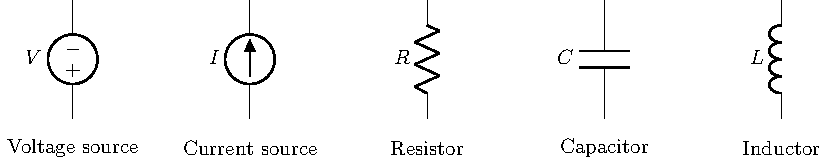
\includegraphics[width=\textwidth]{figure/fig02-01.pdf}
    \caption{Basic circuit elements: voltage source, current source, resistor, capacitor, and inductor.}
    \label{fig:02-01}
\end{figure}

\noindent\textbf{Independent Voltage source.} An idea voltage source provides a fixed voltage $V$ between its two terminals, and can provide any amount of current. Notice that the voltage $V$ can be fixed or time varying. For example, for a DC vortlage source with $V = 5V$, the voltage across the two terminals will be $5V$ for all time. But for a time varying AC source, $V = 5 \sin \left( 100\pi t \right)$, the voltage across its terminal will vary with time. We will often drop the adjective "independent" when we are sure that the context is clear. We will look at dependent sources later, and we will always use the adjective "dependent" to refer to them.

\noindent \textbf{Independent Current source.} An ideal cuyrrent source provide a fixed amount of current to flow throgh its terminals (out through one and in through the other), irrespective of the voltage across its terminals. Current sources can also be time-varying.

\noindent \textbf{Resistor.} A passive element where the current $i_R$ flowing through the element is proportional to the voltage $v_R$ across its terminals.
\[ v_R \propto i_R \]
In the case of linear resistors, the proportionality factor is constant, resulting in Ohm's law,
\begin{equation}
    v_R = R \, i_R
    \label{eq:ch02-01}
\end{equation}

The units of $R$ are $V.A^{-1}$ or $Omhs \left( \Omega \right)$. $R$ is in general positive. The power absorbed by a resistor is given by the product of the voltage across it and the current flowing through the resistor, 
\begin{equation}
    P = v_R \, i_R = i_R^2 \, R = \frac{v_R^2}{R}
    \label{eq:ch02-02}
\end{equation}
This power is dissipated as heat by the resistor. Note that the power absorbed by a resistor is always positive, since $R$ is positive.

We will later see non-linear resistors, where the resistance varies as a function of the applied votlage, temperature and other factors. 

\noindent \textbf{Capacitor.} A capacitor is another passive element with the following voltage current relationship.
\begin{equation}
    i_C = C \frac{d v_C}{dt}
    \label{eq:ch02-03}
\end{equation}

The current $i_C$ through the capacitor is proportional to the rate of change of voltage across its terminals $v_C$. The proportionality factor is called the capacitance $C$, and has units of $F$ (Farads) or $C \cdot V^{-1}$. The voltage across the capacitor is given by at any given time is proportional to the integral of the current flowing through itor the charge stored in the capacitor. The voltage across the capacitor is given by
\begin{equation}
    q = C \, v_C
    \label{eq:ch02-04}
\end{equation}

The instantaneous power absorbed by the capacitor is given by,
\begin{equation}
    P = v_C \, i_C = C \, v_C \frac{d v_C}{dt}
    \label{eq:ch02-05}
\end{equation}

The power absorbed by the capacitor can be positive or negative, depending on the direction of current flow. If the current is flowing into the capacitor, then the voltage across it is increasing, and the power absorbed is positive. If the current is flowing out of the capacitor, then the voltage across it is decreasing, and the power absorbed is negative. A capacitor stores energy in the electric field between its plates. The energy stored in a capacitance at any given time depends on the charge stored in it, and is given by,
\begin{equation}
    E = \frac{1}{2}  C \, v_C^2
    \label{eq:ch02-06}
\end{equation}

\noindent \textbf{Inductor.} An inductor is another passive element with the following voltage current relationship.
\begin{equation}
    v_L = L \frac{di_L}{dt}
    \label{eq:ch02-07}
\end{equation}

The voltage $v_L$ across the inductor is proportional to the rate of change of current $i_L$ flowing through it. The proportionality factor is called the inductance $L$, and has units of $H$ (Henries) or $V \cdot s \cdot A^{-1}$. The current through the inductor is given by at any given time is proportional to the integral of the voltage across it. The current through the inductor is given by
\begin{equation}
    i_L = \frac{1}{L} \int v_L \, dt
    \label{eq:ch02-08}
\end{equation}

The instantaneous power absorbed by the inductor is given by,
\begin{equation}
    P = v_L \, i_L = L \, i_L \frac{di_L}{dt}
    \label{eq:ch02-09}
\end{equation}

The power absorbed by the inductor can be positive or negative, depending on the direction of current flow. If the current is flowing into the inductor, then the voltage across it is increasing, and the power absorbed is positive. If the current is flowing out of the inductor, then the voltage across it is decreasing, and the power absorbed is negative. An inductor stores energy in the magnetic field around it. The energy stored in an inductor at any given time depends on the current flowing through it, and is given by,
\begin{equation}
    E = \frac{1}{2}  L \, i_L^2
    \label{eq:ch02-10}
\end{equation}

\subsection{Kirchoff's Laws}
The five elements alone are not that interesting. But interesting things can be done by connecting these elements together in different ways to form an electrical circuit. The elements are connected together by wires, whicha are assumed to be perfect conductors, i.e. zero resistance. Consider the following circuit (Figure \ref{fig:02-01}),
\begin{figure}[t]
    \centering
    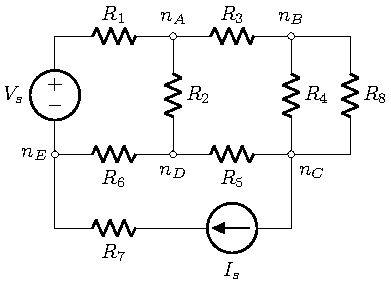
\includegraphics[width=0.5\textwidth]{figure/fig02-02.pdf}
    \caption{A simple electrical circuit with a voltage sourse, a current source, and a bunch of resistors.}
    \label{fig:02-02}
\end{figure}

How do we find out the voltages and currents in the circuit? Kirchoff's laws can be used for analysing such circuits, which are based on the conservation of charge and energy. The circuit in Figure \ref{fig:02-02} is a simple electrical circuit with a voltage source, a current source, and a bunch of resistors. The voltage source provides a fixed voltage $V_s$ between its two terminals, and the current source provides a fixed amount of current $I_s$ to flow through its terminals. The voltages and currents in the rest of the elements will be determined by Kirchoff's laws with the constraints imposed by the voltage and current sources. The two laws are:

\begin{enumerate}
    \item \textbf{Kirchoff's current law (KCL):} The sum of the currents entering a node is equal to the sum of the currents leaving the node. A \textit{node} is a point at which two or more circuit elements are connected together. In Figure \ref{fig:02-02}, $n_A$, $n_B$, $n_C$ and $n_D$ are examples of nodes where three elements are connected together. There are three other nodes in the circuit, can you identify them? 
    
    The sum of the currents at a node is equal to zero. This is based on the conservation of charge, and can be expressed mathematically as:
    \begin{equation}
        \sum_{i=1}^{n} i_i = 0
        \label{eq:ch02-11}
    \end{equation}
    where $i_i$ is the current flowing into or out of the node, and $n$ is the number of elements connected to the node. The current flowing into a node is positive, and the current flowing out of a node is negative.
    
    \item \textbf{Kirchoff's voltage law (KVL):} The sum of the voltages around a closed loop in a circuit is equal to zero. A \textit{closed loop} is a path in the circuit that starts and ends at the same node, and does not cross itself. In Figure \ref{fig:02-02}, the path starting from $n_A$, to $n_D$, to $n_B$, and back to $n_A$ is a closed path. This path invludes the resistors $R_3$, $R_4$, $R_5$, and $R_2$. 
    
    This is based on the conservation of energy, and can be expressed mathematically as:
    \begin{equation}
        \sum_{i=1}^{n} v_i = 0
        \label{eq:ch02-12}
    \end{equation}
    where $v_i$ is the voltage across each element in the loop, and $n$ is the number of elements in the loop.

    The voltage across an element is positive if the current is flowing into the positive terminal of the element, and negative if the current is flowing out of the positive terminal of the element.
\end{enumerate}

Note that the two laws apply for any type of circuit element used in the circuits, independnet or dependent voltage/current sources, resistors, capacitors, inductors, other two, three or four terminal elements.

\subsection{Series and Parallel Connections}
Two elements that share the same voltage across them between a given pair of notes are said to be \textbf{parallel} to each other. In Figure~\ref{fig:02-02}, $R_4$ and $R_8$ are parallel to each other. In a single loop, two elements that share the same current are said to be in \textbf{series} with each other. In Figure~\ref{fig:02-02}, $V_s$ and $R_1$ are in series, $I_s$ and $R_7$ are in series.

\subsubsection{Resistors in series and parallel}
When $n$ resistors $R_1, R_2, \cdots R_n \geq 0$ are in series, these can be combined to an equivalent resistor with resistance $R_{eq}$ given by the following,
\begin{equation}
    R_{eq} = \sum_{i=1}^{n} R_i \implies R_{eq} \geq \max_{1 \leq i \leq n} R_i.
    \label{eq:02-13}
\end{equation}
Note that in a series connection the equivalent resistance is at least as large as the largest value of $R_1$ to $R_n$.

When $n$ resistors $R_1, R_2, \cdots R_n \geq 0$ are in parallel, these can be combined to an equivalent resistor with resistance $R_{eq}$ given by the following,
\begin{equation}
    \frac{1}{R_{eq}} = \sum_{i=1}^{n} \frac{1}{R_i} \implies R_{eq} = \frac{R_1R_2\cdots R_n}{R_1 + R_2 + \cdots + R_n} \implies R_{eq} \leq \min_{1 \leq i \leq n} R_i
    \label{eq:02-14}
\end{equation}
Note that in a parallel connection, the equivalent resistance cannot be larger than the smallest value of $R_1$ to $R_n$.

\subsubsection{Capacitors in series and parallel}
\noindent\textbf{Series connection} of $n$ capacitors $C_1, C_2, \cdots C_n \geq 0$
\begin{equation}
    C_{eq} = \frac{C_1C_2\cdots C_n}{C_1 + C_2 + \cdots + C_n}
    \label{eq:02-15}
\end{equation}

\noindent\textbf{Parallel connection} of $n$ capacitors $C_1, C_2, \cdots C_n \geq 0$
\begin{equation}
    C_{eq} = C_1 + C_2 + \cdots + C_n
    \label{eq:02-16}
\end{equation}

\subsubsection{Inductors in series and parallel}
\noindent\textbf{Series connection} of $n$ capacitors $L_1, L_2, \cdots L_n \geq 0$
\begin{equation}
    L_{eq} = L_1 + L_2 + \cdots + L_n
    \label{eq:02-17}
\end{equation}

\noindent\textbf{Parallel connection} of $n$ capacitors $L_1, L_2, \cdots L_n \geq 0$
\begin{equation}
    L_{eq} = \frac{L_1L_2\cdots L_n}{L_1 + L_2 + \cdots + L_n}
    \label{eq:02-18}
\end{equation}
Its left as an exercise for you to verify these expressions.

\noindent\textbf{What does the equivalent resistance actually mean?} The equilvant resistor with resistance $R_{eq}$ has the same voltage-current relationship as the individual elements in series or parallel connection. We can replace the series or parallel connection of the individual resistors $R_1$ to $R_n$ by a single resistor with value $R_{eq}$ without changing the volatage current relationships in the circuit. The same argument applies for equivalent capacitors and inductors.

\subsubsection{Voltage sources in series and parallel}
\noindent\textbf{Series connection} of $n$ voltage sources $V_1, V_2, \cdots V_n$ will result in an equivalent voltage source $V_{eq}$ given by
\begin{equation}
    V_{eq} = V_1 + V_2 + \cdots + V_n
    \label{eq:02-19}
\end{equation}
Voltage soruces should not be connected in parallel, as this will result in a short circuit. Ideally, an infinite currelt will flow through the connection, because the volaage sources force a potential difference between the two end of the wires and it has zero resistance. Parallel connections are allowed only when the two sources have the same voltage and polarity.

\subsubsection{Current sources in series and parallel}
\noindent\textbf{Parallel connection} of $n$ current sources $I_1, I_2, \cdots I_n$ will
result in an equivalent current source $I_{eq}$ given by
\begin{equation}
    I_{eq} = I_1 + I_2 + \cdots + I_n
    \label{eq:02-20}
\end{equation}
Current sources should not be connected in series; series connections are allowed only when the two sources have the same current and polarity.

\subsection{Superposition Principle}
Linear approximations of circuits are often employed as first order approximations when analysing circuits. A linear ciruit is one that consists of linear passive elements, independent sources and linear dependent sources. Linear circuits follow the superposition principle, which states that the response of a linear circuit to a linear combination of inputs is equal to the corresponding linear comibnation of the responses to each input applied separately. Solving the following circuit (Figure~\ref{fig:02-03}) should make this concept clear.
\begin{figure}[t]
    \centering
    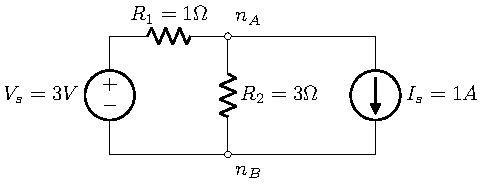
\includegraphics[width=0.65\textwidth]{figure/fig02-03.pdf}
    \caption{A simple circuit with two sourcers}
    \label{fig:02-03}
\end{figure}
For the circuit in Figure~\ref{fig:02-03}, perform the following calculation and compare your results.

\noindent\textbf{Step 1.} Solve for the voltage across and the current through the resistors $R_1$ and $R_2$; we will refer to these are $v_{R1}, i_{R1}$ and $v_{R2}, i_{R2}$, respectively. You should use both Kirchoff's current and voltages laws to compute these variables.

\noindent Let's now consider of the sources in the circuit seperately. This would mean making the source values ``zero''. This corresponds to two different operations on the circuit. Zeroing a voltage source corresponds to replacing it with a wire (a short circuit), while zeroing a current source corresponds to simple removing the current source (an open circuit). 

\noindent\textbf{Step 2.} Zero the voltage source $V_s$ and compute the voltages and currents associated with the two resistors. We will refer to these as $v_{R1,V_s=0}$, $v_{R2,V_s=0}$, $i_{R1,V_s=0}$, and $i_{R2,V_s=0}$.

\noindent\textbf{Step 3.} Zero the current source $I_s$ and compute the voltages and currents associated with the two resistors. We will refer to these as $v_{R1,I_s=0}$, $v_{R2,I_s=0}$, $i_{R1,I_s=0}$, and $i_{R2,I_s=0}$.

\noindent\textbf{Step 4.} For a linear circuit, shown in Figure~\ref{fig:02-03}, the following will always be true.
\begin{equation}
    \begin{split}
        v_{R1} &= v_{R1,V_s=0} + v_{R1,I_s=0}\\
        v_{R2} &= v_{R2,V_s=0} + v_{R2,I_s=0}\\
        i_{R1} &= i_{R1,i_s=0} + i_{R1,I_s=0}\\
        i_{R2} &= i_{R2,i_s=0} + i_{R2,I_s=0}\\
    \end{split}
    \label{eq:02-21}
\end{equation}

\noindent Let's assume that I am only interested in $i_{R2}$. Can I use $i_{R2,V_s=0}$ and $i_{R2,I_s=0}$ to compute the current $i_{R2}$ if $V_s = 1V$ and $I_s=-2A$? 

\subsection{Practical Voltage and Current Sources}
The independent voltage and current sources we have discussed so far are ``ideal'' sources. Practical or real sources do not behave like them - a battery cannot provide any amount of current for a load without any changes to the voltage across its terminals.

A good model of practical voltage source is an ideal voltage source $V_s$ in series with a \textit{internal}, \textit{source} or \textit{output} resistor $R_s$. And for a practical current source, it is an ideal current source $I_s$ in parallel with a resistor $R_s$. The voltage across the terminal of a voltage source as function of the current draw from it is depicted for an ideal and practical voltage source in Figure~\ref{fig:02-04}. For the ideal source (Figure~\ref{fig:02-04a}), the voltage $v_L$ is independent of the current $i_L$ drawn from it. For the practical voltage source (Figure~\ref{fig:02-04b}), the voltage across the terminals is a function of the current drawn from it,
\begin{equation}
    v_L = V_s - R_s \, i_L
    \label{eq:02-22}
\end{equation}
When $R_L = \infty$ ($i_L = 0$), the voltage across the terminals is equal to the voltage of the source $V_s$. This is maximum voltage the practical source can provide. This is also know as the \textit{open circuit voltage} $v_{oc}$ of the source. When $R_L = 0$ ($v_L = 0$), the current drawn from the source $i_L = \frac{V_s}{R_s}$. This is the maximum current the voltage source can provide. This is also known as the \textit{short circuit current} $i_{sc}$ of the source.

\begin{figure}[t]
    \centering
    \begin{subfigure}{0.48\textwidth}
        \centering
        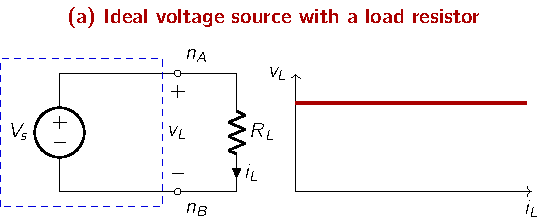
\includegraphics[width=\textwidth]{figure/fig02-04a.pdf}
        \caption{Ideal voltage source}
        \label{fig:02-04a}
    \end{subfigure}
    \hfill
    \begin{subfigure}{0.48\textwidth}
        \centering
        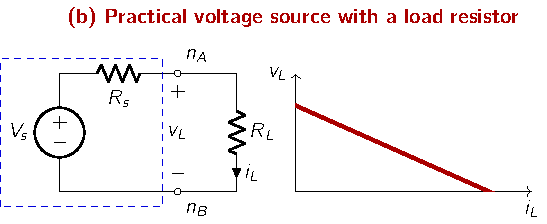
\includegraphics[width=\textwidth]{figure/fig02-04b.pdf}
        \caption{Practical voltage source with a load}
        \label{fig:02-04b}
    \end{subfigure}
    \caption{Comparison of the voltage-current relationship of an ideal and a practical voltage source.}
    \label{fig:02-04}
\end{figure}

\begin{boxedstuff}
    \begin{problem}
        Plot the voltage-current relationship of a practical current source with $I_s = 2A$ and $R_s = 10\Omega$. What are $v_{oc}$ and $i_{sc}$?
    \end{problem}
\end{boxedstuff}

\subsection{Thevenin's and Norton's Theorems}
Thevenin's and Norton's theorems are two important theorems in circuit theory that allow us to simplify complex circuits into simpler equivalent circuits. These theorems are based on the superposition principle, and can be used to analyze linear circuits with independent and dependent sources.

\noindent\textbf{Thevenin's Theorem.} Thevenin's theorem states that any linear circuit with independent and dependent sources can be replaced by an equivalent circuit with a single voltage source $V_{th}$ in series with a resistor $R_{th}$, connected to the load resistor $R_L$. 

\noindent\textbf{Norton's Theorem.} Norton's theorem states that any linear circuit with independent and dependent sources can be replaced by an equivalent circuit with a single current source $I_{N}$ in parallel with a resistor $R_{N}$, connected to the load resistor $R_L$.
\begin{figure}[t]
    \centering
    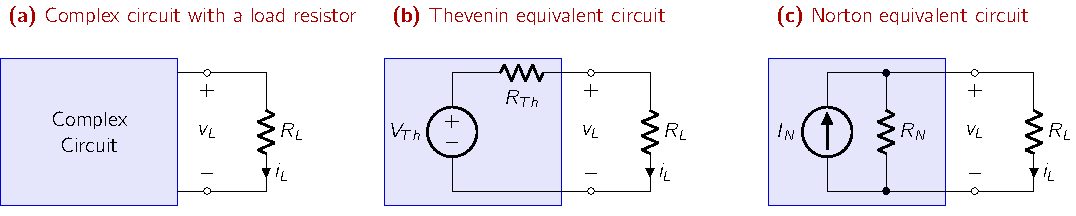
\includegraphics[width=\textwidth]{figure/fig02-05.pdf}
    \caption{Thevenin's and Norton's circuits for a complex linear circuit. The Thevenin and Norton equivalent circuits have the same voltage-current relationship for any load.}
    \label{fig:02-05}
\end{figure}

\noindent\textbf{Computing the Thevenin and Norton equivalent circuits.} The Thevenin and Norton equivalent circuits can be computed using the following steps:
\begin{enumerate}
    \item Remove the load resistor $R_L$ from the circuit.
    \item Compute the open circuit voltage $v_{oc}$ across the terminals of the load resistor. This is the Thevenin voltage $V_{th}$. This can be using the superposition principle, where we zero all the independent sources except one and compute the open circuit voltage. The overall open circuit voltage is the sum of the open circuit voltages when all other sources are zeroed.
    \item Compute the short circuit current $i_{sc}$ through the terminals of the load resistor. This is the Norton current $I_{N}$. This too can be calculated using the superposition principle.
    \item Compute the Thevenin resistance $R_{th}$ by zeroing all independent sources in the circuit and computing the equivalent resistance seen from the terminals of the load resistor (without the load resistor). This is also equal to the Norton resistance $R_{N}$.
    \item The Thevenin and Norton equivalent circuits are then given by:
    \begin{equation}
        \begin{split}
            V_{th} &= v_{oc}\\
            I_{N} &= i_{sc}\\
            R_{th} &= R_{N}
        \end{split}
        \label{eq:02-23}
    \end{equation}
    \item The load resistor $R_L$ can be connected to either the Thevenin or Norton equivalent circuit, and the voltage and current across it can be computed using the voltage-current relationship of the equivalent circuit.
\end{enumerate}

\begin{boxedstuff}
    \begin{problem}
        Compute the Thevenin and Norton equivalent circuits for the circuit shown in Figur~\ref{fig:02-02} assuming the following as the load resistor: (a) $R_8$; (b) $R_2$; and (c) $R_7$.
    \end{problem}
\end{boxedstuff}

\subsection{Maximum Power Transfer Theorem}
The maximum power transfer theorem states that the maximum power is transferred to the load resistor $R_L$ when the load resistance is equal to the Thevenin resistance $R_{th}$ of the circuit. Consider the following circuit (Figure~\ref{fig:02-06}). The power absorbed by the load resistor $R_L$ is given by,
\begin{equation}
    P_{R_L} = \frac{R_L}{(R_{th} + R_L)^2} \, V_{th}^2
    \label{eq:02-24}
\end{equation}
Its easy to check that the optimal value of $R_L$ that maximizes the power absorbed by the load resistor is given by,
\begin{equation}
    \begin{split}
        R_L^* &= \arg\max_{R_L} \,\, \frac{R_L}{(R_{th} + R_L)^2} \, V_{th}^2 = R_{Th} \\
        P_L^* &= \max_{R_L} \,\, \frac{R_L}{(R_{th} + R_L)^2} \, V_{th}^2 = \frac{1}{4}\left(\frac{V_{Th}^2}{R_{Th}}\right)
    \end{split}
    \label{eq:02-25}
\end{equation}

\begin{figure}[t]
    \centering
    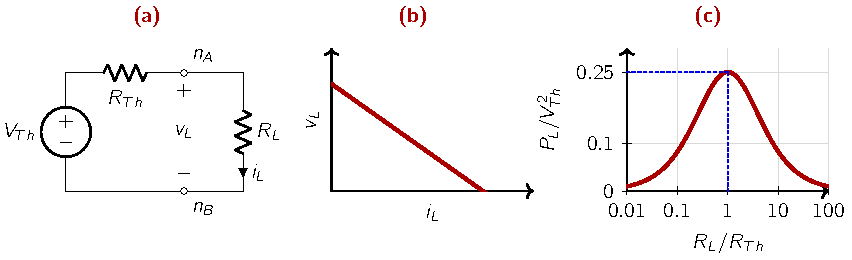
\includegraphics[width=\textwidth]{figure/fig02-06.pdf}
    \caption{Maximum power transfer theorem.}
    \label{fig:02-06}
\end{figure}

\begin{boxedstuff}
    \begin{problem}
        Prove the statements in Eq.~\ref{eq:02-25}. (\textit{Hint:} Use the first order condition for maximization of a continuous function.)
    \end{problem}
\end{boxedstuff}



% \begin{tikzpicture}
%     \draw (2.5, 0) node [npn] (t) {$Q_1$};
%     \draw (0, 0) node[ocirc] {} to[R, l=$R_1$] (t.base);
%     \draw (t.collector) to[R, l=$R_2$] ++(0, 2) -- ++(1.5, 0) node[ocirc] (p1){};
%     \draw (t.collector) node[circ] {} -- ++(1.5, 0) node[ocirc] (p2) {};
%     \draw (t.emitter) -- ++(0, -1) node[circ] (e){} -- ++ (1.5, 0) node[ocirc] (p3) {};
%     \draw (e.center) -- ++(-2.5, 0) node[ocirc]{};
%     \draw [-latex] ([xshift=-2mm]0, 0) -- ++(0, -1.8) node[midway, left] {$U_1$};
%     \draw [-latex] ([xshift=2mm]p2.center) -- ([xshift=2mm]p3.center) node[midway, left] {$U_3$};
%     \draw (t.base) node [above] {B};
%     \draw (t.collector) node [left] {C};
%     \draw (t.emitter) node [left] {E};
% \end{tikzpicture}



% \input{./chapter/01-matrices.tex}
% \input{./chapter/01-lineartransf.tex}
% \input{./chapter/01-lineqsolve.tex}
% \input{./chapter/01-orthogonality.tex}
% \input{./chapter/01-matrixinverses.tex}
% 05 matrix inverses
% 06 eigenvalues and eigenvectors
% 07 positive definite matrices
% 08 singular value decomposition

% \part{Optimization}
% % 09 mathe
% \part{Probability and Statistics}
% \input{./chapter/03-02statsest.tex}
% % \part{Least Squares}

% \part{Linear Programming}
% \input{./chapter/04-01linearprogramming.tex}

% \part{Computer Science}
% % \input{./chapter/complexity.tex}
% % !TEX root = ../notes_template.tex
\chapter{Machine Learning}\label{chp:machine_learning}
\minitoc

\section{Regression}
% \gls{algorithm};
\subsection{Gradient descent}\label{sec:gradient_descent}
\gls{gd};
% \glsxtrshort{gd}

\section{Support Vector Machine}
\gls{svm};
% % \input{./chapter/algorithms.tex}

% \part{Physics}
% % !TEX root = ../notes_template.tex
\chapter{Quantum Mechanics}\label{chp:quantum_mechanics}
\minitoc

\section{Hamiltonian}
\gls{hamiltonian};
% \glsxtrshort{qm};

\section{Path Integral}
\gls{lagrangian}

\section{Quantum Field Theory}
\gls{qft};
% % \input{./chapter/quantum_field_theory.tex}

% \begin{appendices}
% % !TEX root = ../notes_template.tex
\chapter{Formulas}

\section{Gaussian distribution}\label{sec:gaussian_distribution}
\begin{definition}[Gaussian distribution]\label{def:gaussian_distribution}
    \myindex{Gaussian distribution}
\end{definition}

\begin{theorem}[Central limit theorem]\label{thm:central_limit_theorem}
\end{theorem}
% \end{appendices}

\backmatter

%%%%%%%%%%%%%%% Reference %%%%%%%%%%%%%%%

\printbibliography[heading=bibintoc]
\printindex

\end{document}

